\section{Design og Implementering}
	Denne sektion indeholder uddybende forklaring af design og implementering.
	Der er brugt MVP design pattern til alle activities, samt dependency injection for at gøre koden testbar, og åben for udvidelser.
	
	\subsection{Log ind}
	Dette afsnit vil indeholde en gennem gang af design, grafisk bruger interface og implentering af Log ind activityen til android applikationen
	\subsubsection{Design}
	I dette afsnit ses et sekvens diagram over log ind forløbet til android applikationen
	\begin{figure} [!ht]
		\begin{center}
			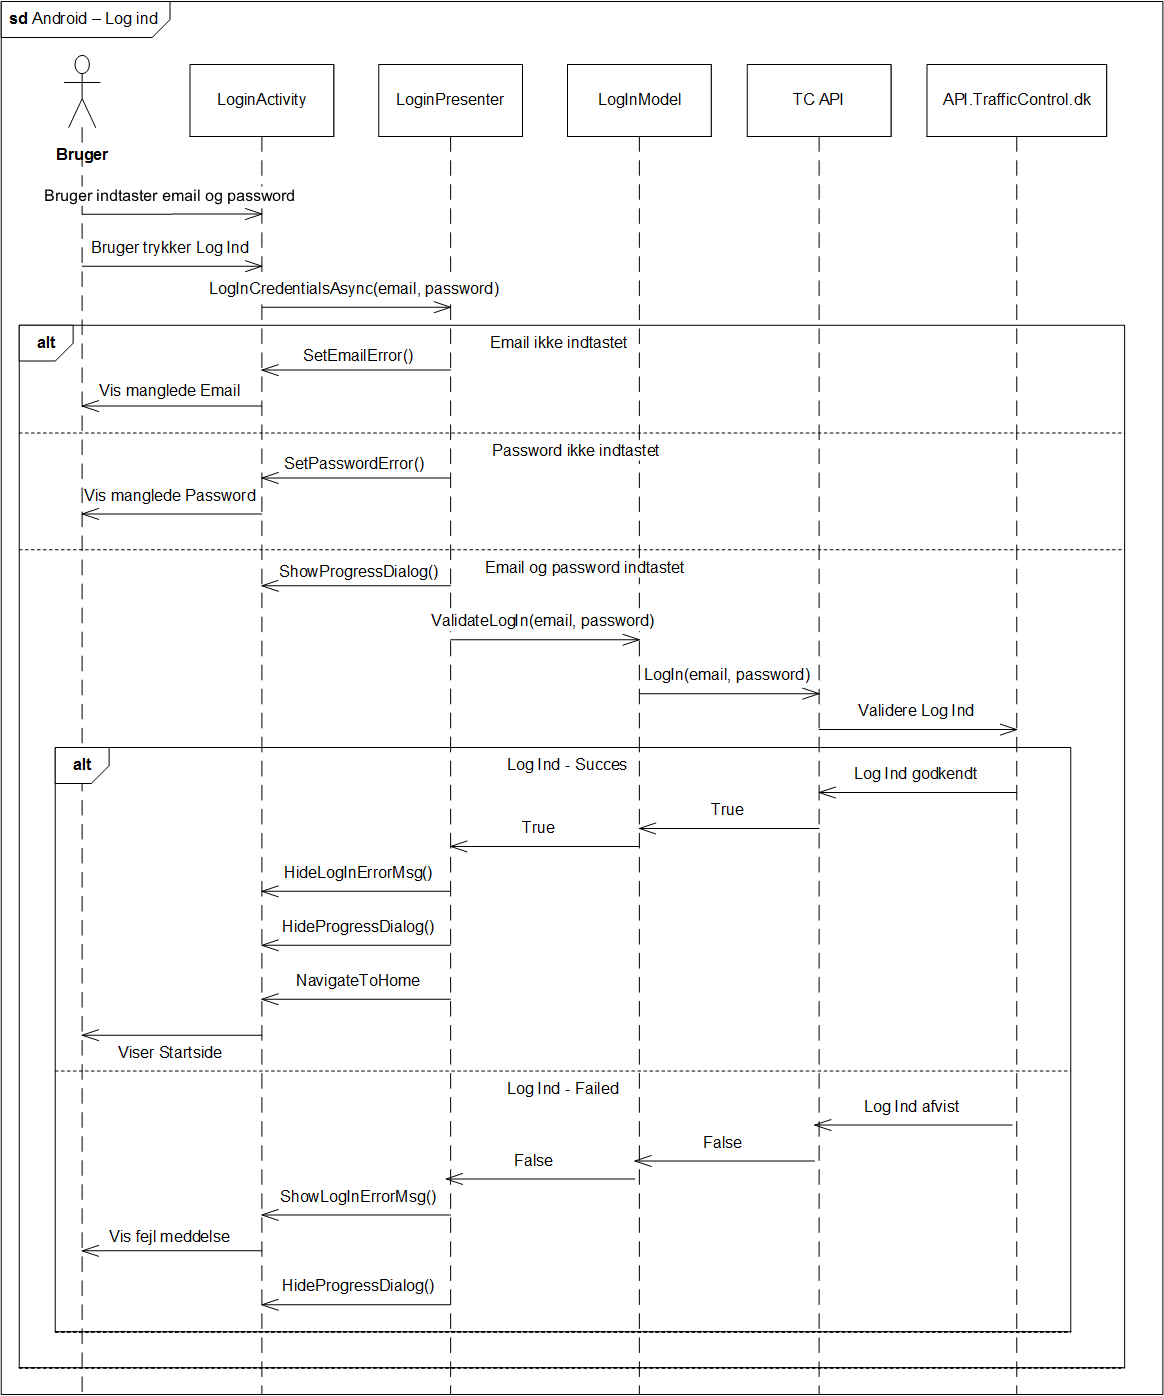
\includegraphics[height=15cm]{Android/Billeder/SekvensDiagramLogInd}
		\end{center}
		\caption{Sekvens diagram for log ind på android applikationen}
		\label{fig:Sekvens diagram for Log Ind Android}
	\end{figure}
	\pagebreak
	
	På figur \ref{fig:Klasse diagram for Log Ind Android} ses hvordan klasserelationerne til Login activiteten er designet, med udgangspunkt i MVP.
	
	\begin{figure} [!ht]
		\begin{center}
			\includegraphics[height=15cm]{Android/Billeder/clLogin}
		\end{center}
		\caption{Klasse diagram for log ind på android applikationen}
		\label{fig:Klasse diagram for Log Ind Android}
	\end{figure}
	\pagebreak
	
	\subsubsection{Grafisk Bruger Interface}
	Her ses hvordan at Log Ind siden ser ud på android applikationen.
	Det er et meget simpelt design, for at gøre det yderst bruger venligt.
	
	\begin{figure} [h]
		\begin{center}
			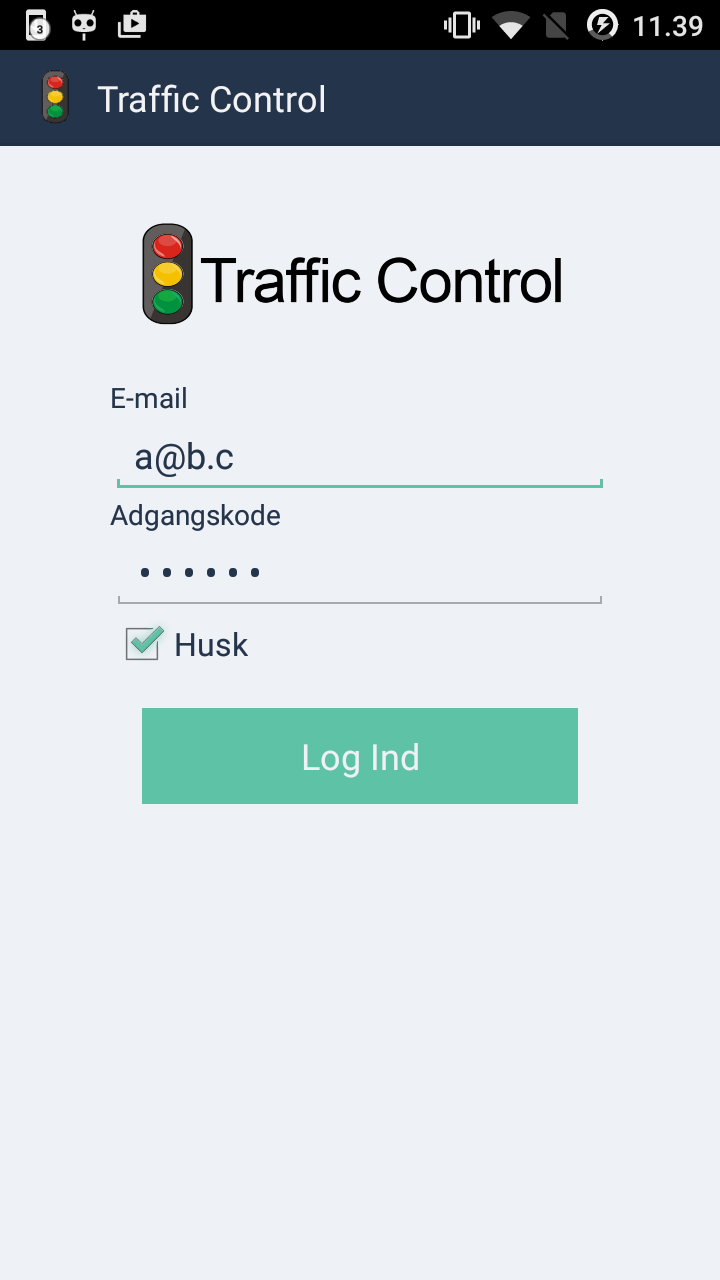
\includegraphics[height=7cm]{Android/Billeder/AndroidLogIn}
		\end{center}
		\caption{Traffic Control - Log ind}
		\label{fig:Traffic Control - Log ind}
	\end{figure}
	
	\subsubsection{Implementering}
	Når en brugen forsøger at logge ind, validerer presenteren at der er indtastet information, inden at informationen bliver sendt videre til modellen. Hvis et felt ikke er udfyldt giver presenteren besked til viewet om at en fejlbesked om dette, skal vises. Hvis alle de påkrævet feltet er fyldt ud bliver et request sendt til API'et, gennem Modellen og DAL-laget. 
	\\Specielt for LogInActivity, benyttes en privat fil på telefonen til at gemme log ind oplysninger. Ansvaret for sikkerheden af denne fil, står Android frameworket for.
	
	\pagebreak